\chapter{Available Modules and How to Use Them}
\label{ch:modules}
% ##################################################################################################################
% ##################################################################################################################

\hfill \textbf{Author:} Andreas Horni

\begin{center} 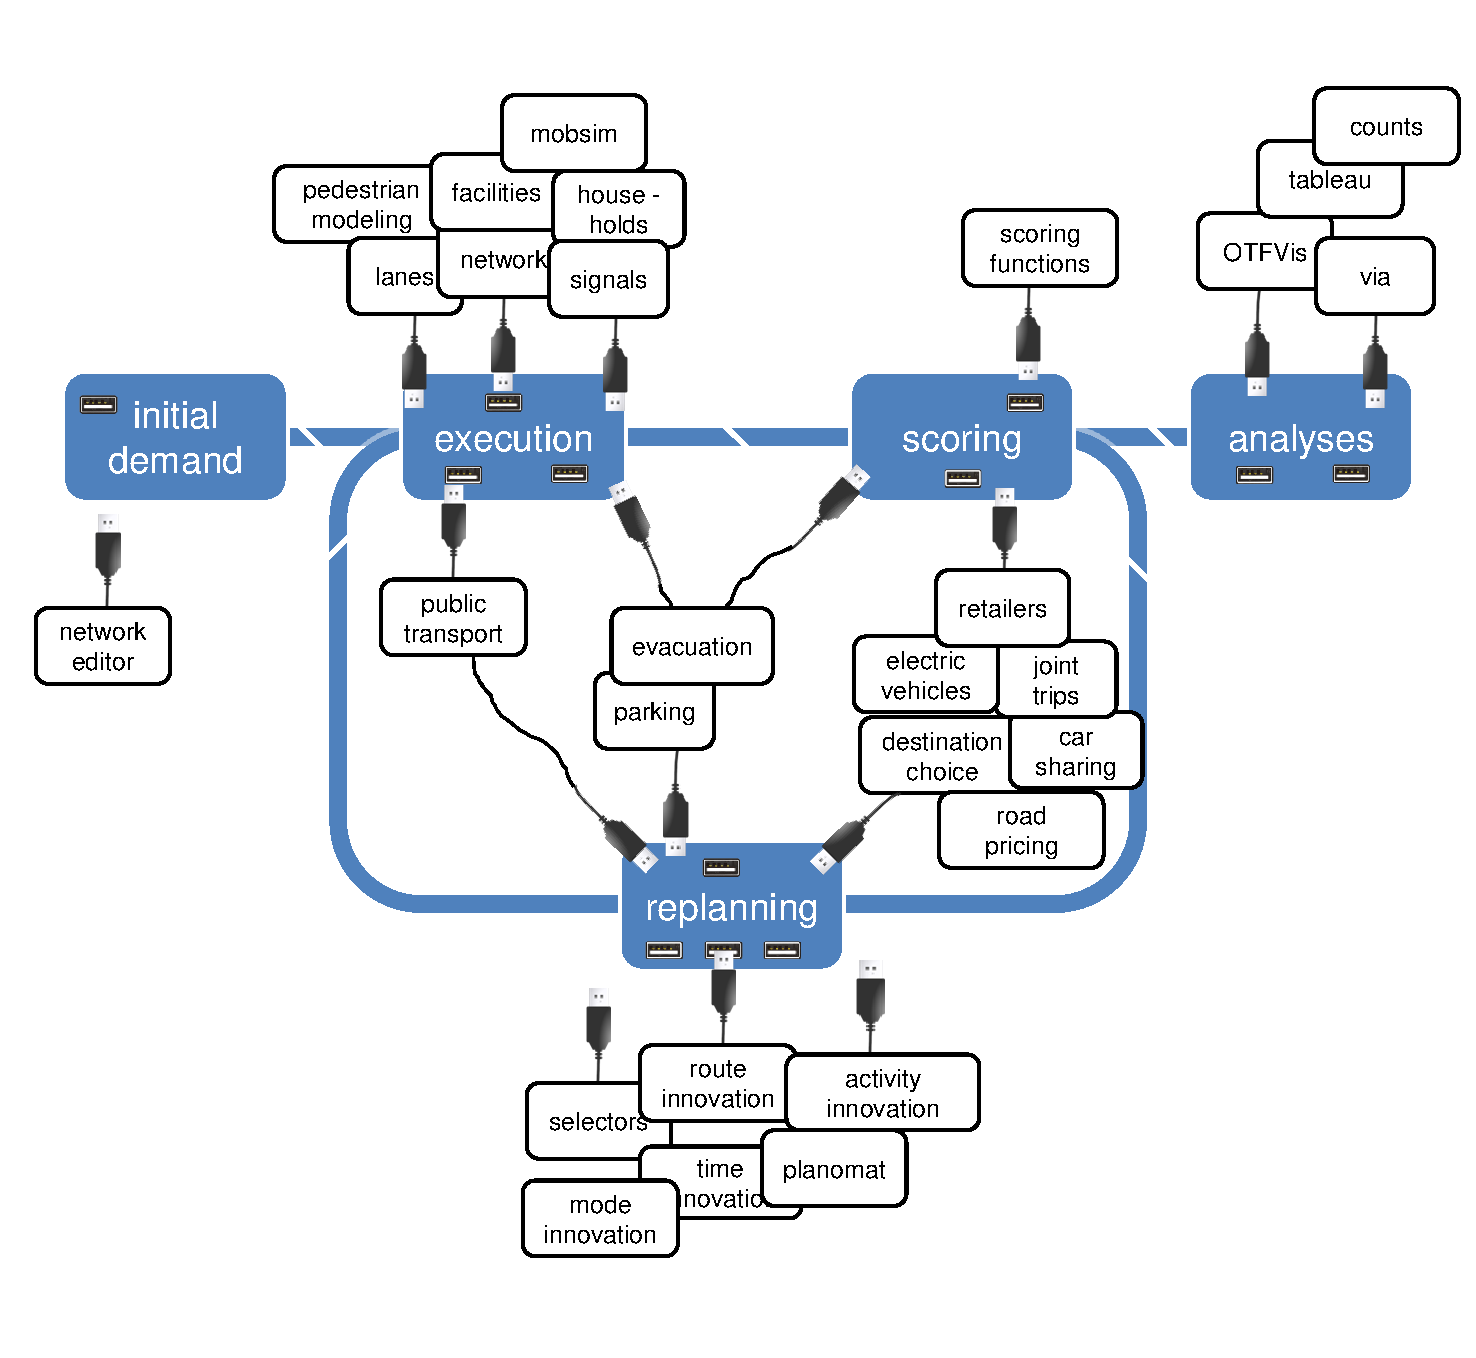
\includegraphics[width=0.5\textwidth, angle=0]{extending/figures/modules.pdf} \end{center}

% ##################################################################################################################
In this chapter you will learn about the possibilities to configure, extend, and customize MATSim by available functionality. In Chapter~\ref{ch:extensionpoints} you will see, how you can hook in your own extensions.

% ##################################################################################################################
\section{MATSim Modules}
The basic concept to extend MATSim is the usage of modules. But, please be aware that when it comes to configuring MATSim the term ``module'' is very extensively used such that a clear definition of what is a module and what is not is not available to date. This consequence of organic grows be corrected on the long run, for now, we try to just sort out the different meanings of the word module. 

Following different components are called modules.

\paragraph{Components in \lstinline|org.matsim|:} % --------------
The term ``module'' is used for components providing distinct functionality, residing in the \lstinline|org.matsim| package and having their own section in the default configuration file. Such a section looks as follows. 
\begin{lstlisting}
<module name="aModule"> 
    <param name="aParameterForAModule0" value="someValueX" /> 
    <param name="aParameterForAModule1" value="someValueY" />  
</module>
\end{lstlisting}

\paragraph{Contributions:} % --------------
The term ``module is furthermore used for contributions, residing in the \lstinline|org.matsim.contrib| package and either having their section in the default configuration file (such as destination choice) or not (such as the wagonsim contribution). 

\paragraph{External Functionality:} % --------------
Also external components plugged in and replacing a MATSim module, such as a mobsim, are called modules.

MATSim provides the possibility that the parameters of arbitrary external modules are added to the configuration file as shown above. In the respective module, the parameters can be accessed with the method \lstinline|public final String findParam(final String moduleName, final String paramName)| of the \lstinline|Config| class.

\paragraph{Standalone Tools:} % --------------
Also the standalone tools referencing MATSim as a library, such as the network editor, or the visualizer via, are termed modules in current practice.

\paragraph{Replanning Modules:} % --------------
A slightly different meaning of modules, which is only relevant for the MATSim developer and API-user, is as follows. In the package package \lstinline|org.matsim.core.replanning.modules| replanning functionality is provided in classes that are derived from \lstinline|AbstractMultithreadedModule|. 

% ===================================================================================
\subsection{Current Problems With Modules}
The majority of the replanning modules have their own section in the configuration file, but some do not, such as the \lstinline|TripsToLegsModule|. In that package---called modules---there are furthermore, the factories for the plan selectors. For the selectors and their factories, it is unclear if they are modules.

To make things worse, there are cases where module names in the configuration file are not (yet) consistent with the naming in the code. Examples are ``\lstinline|strategy|'' in the configuration file and ``\lstinline|StrategyManager|'' in the code, or ``strategy module'' in the config file and ``\lstinline|PlanStrategy|'' in the code \ah{Nochmals nachsehen!}. Furthermore, modules are atomic. There is, for example, a module called ``\lstinline|ChangeSingleLegMod|'', a module ``\lstinline|ChangeLegMode|'' and a module ``\lstinline|SubtourModeChoic|'' instead of one single module called ``\lstinline|ModeChoice|''. This, on the one hand, has historical reasons; the three modules were developed temporally separated. On the other hand, the parameter set for a module is only minimal and unambiguous if provided for atomic modules as different parameters are required for the three modules.

For the presentation of the available functionality, we chose to not use a single section per module but to group them according to common transport planning categories, in the example above this would be ``mode choice'' instead of the atomic categories, where we use terms ``functionality'' for the larger categories and ``module'' for the atomic components. 

Due to the distributed and project- and dissertation-driven MATSim contribution process (see Chapter \ref{ch:developmentprocess} modules are usually implemented for a specific practical purpose leading to various limitations of the respective module, e.g., modules might only work for a specific mode or for a defined calling order. Before, an additional effort is undertaken to generalize the module toward its embedding in the complete framework, the combination of a specific module with other functionality remains a non-straight-forward task. This means, that the user is in charge of systematically testing a specific modules combination before productively applying it.

% ##################################################################################################################
\section{An Overview of Existing Modules}
Figure~\ref{fig:matsimmodules} shows where in the MATSim loop, common MATSim modules can be plugged in. The technical details for their usage, in particular the parameter sets are described in \citep[][]{MATSim_Userguide_2014} and in the javadoc.
%
\createfigure%
{MATSim functionality}%
{MATSim functionality}%
{\label{fig:matsimmodules}}%
{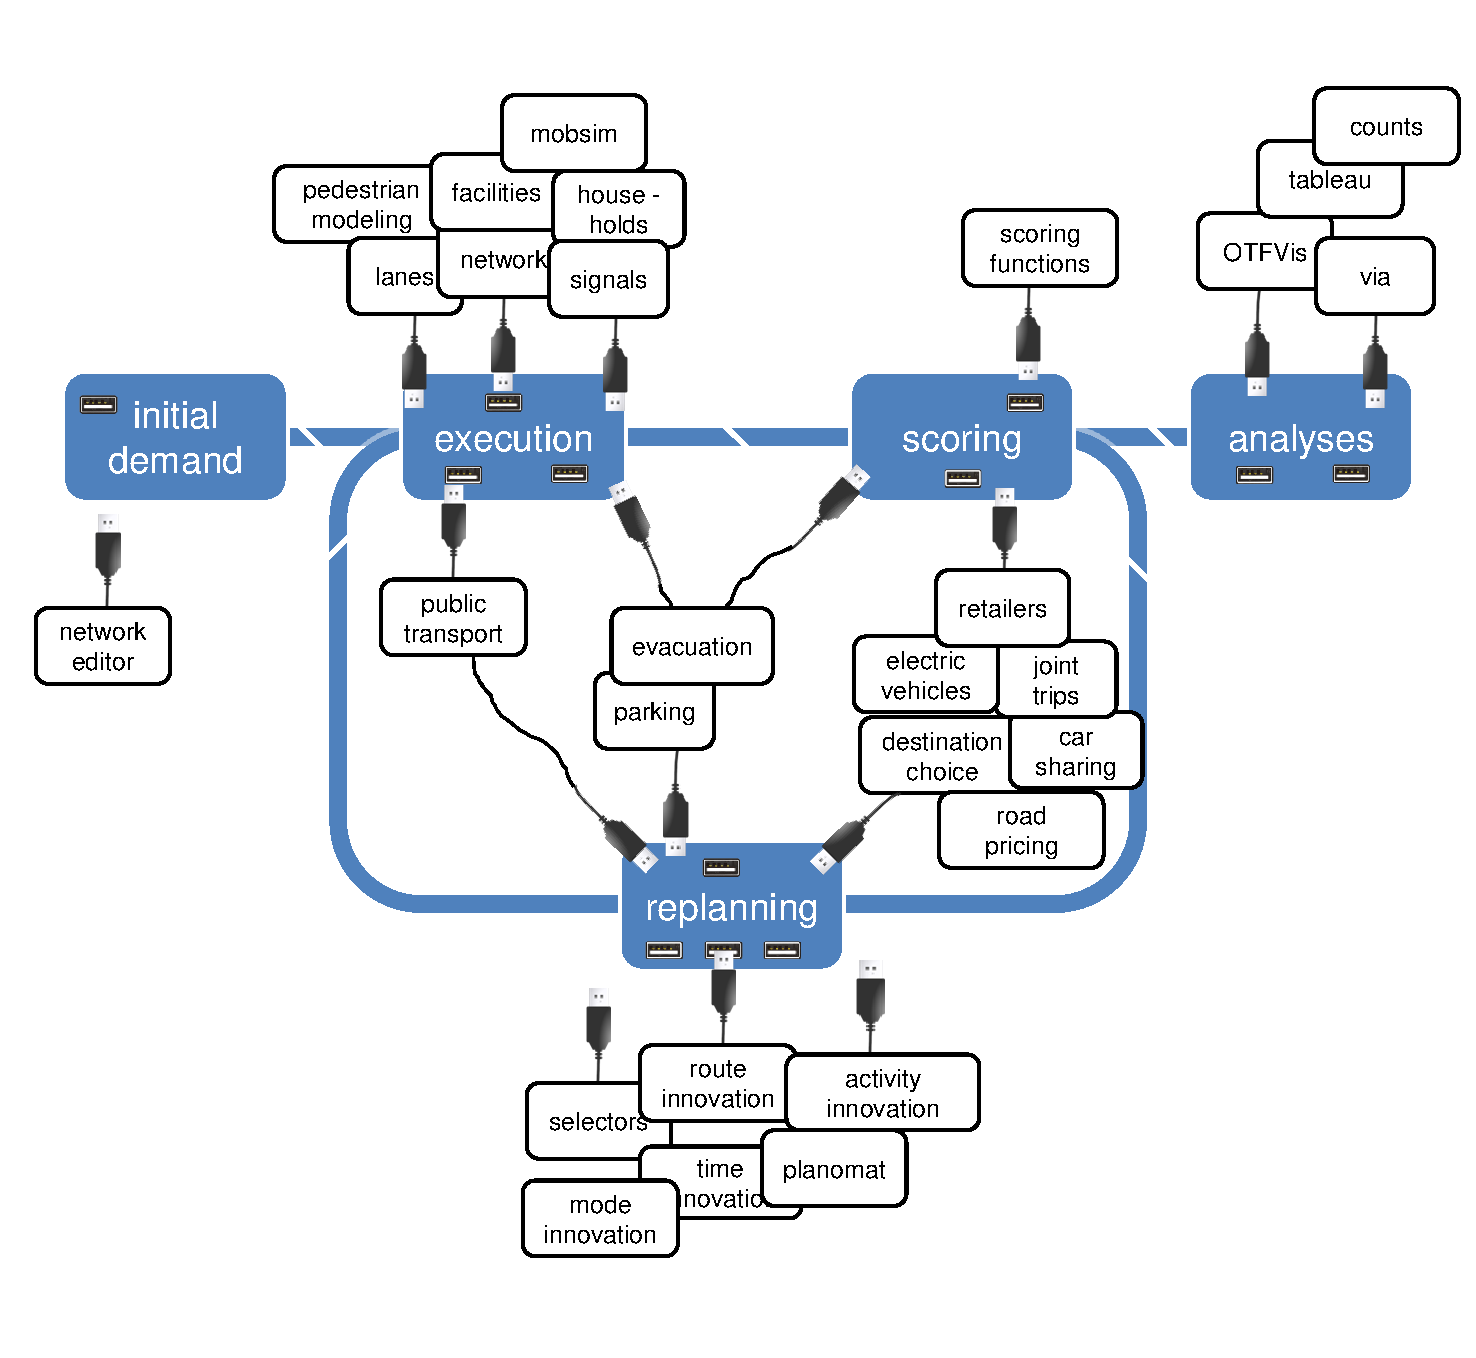
\includegraphics[width=0.99\textwidth, angle=0]{extending/figures/modules.pdf}}%
{}
%
The description of the modules in this and the following chapters is based on following categorization.
%
\createtable%
{Modules}%
{Modules}%
{\label{tab:modules}}%
{%
  \begin{tabular}[c]{|l|l|}
	\hline
	\textbf{Strategy Modules} & Section~\ref{sec:strategymodules} \\
	\hline
	Time Choice & Section~\ref{sec:timechoice} \\
	Route Choice & Section~\ref{sec:routechoice} \\
	Mode Choice & Section~\ref{sec:modechoice} \\
	Selectors & Section~\ref{sec:selectors} \\
	Destination Choice & Chapter~\ref{ch:destinationchoice} \\
	\hline
	\textbf{Further Choice Modules} & Section~\ref{sec:furtherchoicemodules} \\
	\hline
	Planomat & Section~\ref{sec:planomat} \\
	Activity Choice a.k.a. PlanomatX & Section~\ref{sec:activitychoice} \\
	Within-day Replanning & Section~\ref{sec:withinday} \\
	\hline
	\textbf{Supply-Side Modules} & Section~\ref{sec:supplysidemodules} \\
	\hline
	Network & Section~\ref{sec:network} \\
	Counts & Section~\ref{sec:counts} \\
	Facilities & Section~\ref{sec:facilities} \\
	Signals and Lanes & Chapter~\ref{ch:signalslanes} \\
	\hline
	\textbf{Demand-Side Modules and Specific Transport Modes Modules} & Section~\ref{sec:dsm} \\
	\hline
	Population & Section~\ref{sec:population} \\
	Households & Section~\ref{sec:households} \\
	Vehicles & Section~\ref{sec:vehicles} \\
	Flight Traffic & Section~\ref{sec:flighttraffic} \\
	Public Transport & Chapter~\ref{ch:pt} \\
	Multi-Modal Simulation & Chapter~\ref{ch:multimodalsim} \\
	Freight Traffic & Chapter~\ref{ch:freight} \\
	Car Sharing & Chapter~\ref{ch:carsharing} \\
	Joint Trips and Social Networks & Chapter~\ref{ch:jointtrips} \\
	Dynamic Transport Systems & Chapter~\ref{ch:dts} \\
	Parking & Chapter~\ref{ch:parking} \\ 
	Electric Vehicles & Chapter~\ref{ch:elvehicles} \\
	\hline
	\textbf{Mobsims} & Section~\ref{sec:mobsims} \\
	\hline
	QSim & Section~\ref{sec:qsim} \\
	queueSimulation & Section~\ref{sec:queueSimulation} \\
	JDEQSim & Section~\ref{sec:jdeqsim} \\
	DEQSim & Section~\ref{sec:deqsim} \\
	\hline
	\end{tabular}
}%
{}
	
\createtable%
{Modules continued}%
{Modules continued}%
{\label{tab:modulescontinued}}%
{%
  \begin{tabular}[c]{|l|l|}
	\hline
	\textbf{General Purpose Modules} & Section\ref{sec:generalpurposemodules} \\
	\hline
	Controler & Section~\ref{sec:controler} \\
	Global & Section~\ref{sec:global} \\
	Scenario & Section~\ref{sec:scenario} \\
	Scoring & Section~\ref{sec:scoring} \\ 
	\hline	
	\textbf{Special Purpose Modules, Tools and Functionalities} & Section~\ref{sec:specialpurpose} \\
	\hline
	Travel Time Calculator & Section~\ref{sec:ttc} \\
	Link Stats & Section~\ref{sec:linkStats} \\
	Parallel Computing & Section~\ref{sec:parallelcomputing} \\
	Landuse & Section~\ref{sec:landuse} \\
	Visualizer OTFVis & Section~\ref{sec:OTFVis} \\
	Visualizer senozon via & Section~\ref{sec:via} \\
	Cadyts & Section~\ref{sec:cadyts} \\
	Extension of Simulation Horizon & Section~\ref{sec:longitudinalscenario} \\
	Warmstart & Section~\ref{sec:warmstart} \\
	Roadpricing & Chapter~\ref{ch:roadpricing} \\
	Emisssions & Chapter~\ref{ch:emissions} \\
	Accessibility & Chapter~\ref{ch:accessibility} \\
	Evacuation & Chapter~\ref{ch:evacuation}  \\
	WagonSim & Chapter~\ref{ch:wagonSim} \\
	PSim & Chapter~\ref{ch:psim} \\
	Network editors &  Chapter~\ref{ch:networkeditor} \\
	Business Analytics & Chapter~\ref{ch:businessanalytics} \\
	\hline
	\end{tabular}
}%
{}

% ##################################################################################################################
\section{Strategy Modules}
\label{sec:strategymodules}
The strategy modules are the basic choice modules available in MATSim. All strategy modules are called by configuring the strategy module in the configuration file as shown in the following example.

\begin{lstlisting}
<module name="strategy" > 
    <param name="ModuleProbability_1" value="0.1" /> 
    <param name="Module_1" value="ChangeLegMode" /> 
    <param name="ModuleProbability_2" value="0.2" /> 
    <param name="Module_2" value="TimeAllocationMutator" /> 
    <param name="ModuleProbability_3" value="0.7" /> 
    <param name="Module_3" value="SelectExpBeta" /> 
</module>
\end{lstlisting}

Strategy modules are numbered, where each module is given a weight which determines the probability by which the course of action represented by the module is taken. In this example, each agent changes his leg mode with probability 0.1, its plan timing with probability 0.2. A strategy module is, in the code, always a combination of a plan selector and zero or more strategy module elements. In the example, the agent choses a plan from his set of plans according to a logit model with probability 0.7. The weights of the strategy modules are renormalized in case they do not sum to one. 

Combining different modules is not straight-forward in MATSim. This important topic urgently awaits future analysis. To begin with, here, the combination of the strategy modules with public transport is presented in Table \ref{tab:combination}.

% ----------------------------------
\createtable%
{Strategy Module Combination}%
{Strategy Module Combination}%
{\label{tab:combination}}%
{%
  \begin{tabular}[c]{|c|c|c|}
   \hline
\textbf{Choice Dimension}	& \textbf{Default Strategy} & \textbf{Public Transport}\\
\hline
time choice & TimeAllocationMutator &  TransitTimeAllocationMutator\\
\hline
route choice & ReRoute & ReRoute \\
\hline
mode choice & \multirow{2}{*}{ChangeLegMode} & \multirow{2}{*}{TransitChangeLegMode} \\
(all legs get same mode) &  &  \\
\hline
mode choice & \multirow{2}{*}{ChangeSingleLegMode} & \multirow{2}{*}{TransitChangeSingleLegMode} \\
(each leg can have a different mode) &  &  \\
\hline
mode choice & \multirow{2}{*}{SubtourModeChoice} & \multirow{2}{*}{TransitSubtourModeChoice} \\
(subtour-based) &  &  \\
\hline
destination choice & LocationChoice & LocationChoice \\
\hline
  \end{tabular}
}%
{}

% ===================================================================================
\subsection{Time Choice}
\label{sec:timechoice}
Time choice is applied by adapting the configuration file strategy module,
%
\begin{lstlisting}
<module name="strategy" > 
    <param name="ModuleProbability_1" value="0.x" /> 
    <param name="Module_1" value="TimeAllocationMutator" /> 
    [...]
</module>
\end{lstlisting}
%
and by defining its parameters in the configuration file time choice section, 
%
\begin{lstlisting}
<module name="TimeAllocationMutator" > 
    <param name="param0" value="value0" /> 
    [...]
</module>
\end{lstlisting}
%
The code for time choice can be found in the class \lstinline|org.matsim.core.replanning.modules.TimeAllocationMutator|

The module shifts activity end times randomly within a configurable range as described by \citet[][]{BalmerEtAl_Timmermans_2005, Raney_PhDThesis_2005, Balmer_unpub_VSP_2004, BalmerEtAl_unpub_EIRASS_2004, BalmerEtAl_unpub_STRC_2004}. A best-reponse approach to time choice is applied by ``planomat'' described in Section \ref{sec:planomat}.

% ===================================================================================
\subsection{Route Choice} 
\label{sec:routechoice}
Route choice is applied by adapting the configuration file strategy module,
%
\begin{lstlisting}
<module name="strategy" > 
    <param name="ModuleProbability_1" value="0.x" /> 
    <param name="Module_1" value="ReRoute" /> 
    [...]
</module>
\end{lstlisting}
%
and by defining its parameters in the configuration file planscalcroute section, 
%
\begin{lstlisting}
<module name="planscalcroute" > 
    <param name="param0" value="value0" /> 
    [...]
</module>
\end{lstlisting}
%
The routing algorithm needs to be specified in the configuration file controler module 
%
\begin{lstlisting}
<module name="planscalcroute" > 
    <param name="routingAlgorithmType" value="{Dijkstra | FastDijkstra | 
    		AStarLandmarks | FastAStarLandmarks}" /> 
    [...]
</module>
\end{lstlisting}
%
MATSim routing is described by \citet[]{LefebvreBalmer_STRC_2007, LefebvreBalmer_TechRep_IVT_2007}. The configuration necessary for public transport is shown in Chapter \ref{ch:ptmodule}.

% ===================================================================================
\subsection{Mode Choice}
\label{sec:modechoice}
Different options exists to perform mode choice. Following modules can be specified in the configuration file strategy module,
%
\begin{lstlisting}
<module name="strategy" > 
    <param name="ModuleProbability_1" value="0.x" /> 
    <param name="Module_1" value="{ChangeLegMode | 
    		ChangeSingleLegMode | SubtourModeChoice}" /> 
    [...]
</module>
\end{lstlisting}
%
and configured in the confuguration file modules with
%
\begin{lstlisting}
<module name="{changeLegMode | 
				changeLegMode | subtourModeChoice}" > 
    <param name="param0" value="value0" /> 
    [...]
</module>
\end{lstlisting}
%
\lstinline|ChangeLegMode| randomly picks one of the plans of a person and changes its mode of transport. By default, the supported modes are driving a car and using public transport. Only one mode of transport per plan is supported. For using different modes for sub-tours on a single day the \lstinline|SubtourModeChoice| module is required. Optionally, car-availability is respected. \lstinline| ChangeSingleLegMode| randomly picks one of the plans of a person and changes the mode of transport of one single leg. The leg is picked randomly. In contrast to \lstinline|ChangeLegMode|, it allows for multiple modes in one plan. By default, the supported modes are driving a car and using public transport. Also, this module is able to (optionally) respect car-availability. 
 
Mode choice is described by \citet[][]{RieserEtAl_TRR_2009, MeisterEtAl_WCTRS_2010, CiariEtAl_STRC_2008, CiariEtAl_STRC_2007}

% ===================================================================================
\subsection{Selectors}
\label{sec:selectors}
Following selectors are available in the configuration file strategy module: 
%
\begin{lstlisting}
<module name="strategy" > 
    <param name="ModuleProbability_1" value="0.x" /> 
    <param name="Module_1" value="{a specific selector}" /> 
    [...]
</module>
\end{lstlisting}
%
%
\begin{itemize}
	\item \lstinline|KeepLastSelected| keeps the plan selected in the previous iteration.
	\item \lstinline|BestScore| selects the plan with the highest score of the previous iteration.
	\item \lstinline|SelectExpBeta| performs multinomial logit model selection between plans.
	\item \lstinline|ChangeExpBeta| changes to a different plan with probability dependent on $e^{\Delta_{score}}$, where $\Delta_{score}$ is the score difference between the two plans. 
	\item \lstinline|SelectRandom| performs random selection between the plans.
	\item \lstinline|SelectPathSizeLogit| selects an existing Plan according to the Path Size Logit described by \citet[][]{FrejingerBierlaire_TransResB_2007}.
\end{itemize}

The implementation of selectors reside in the \lstinline|package org.matsim.core.replanning.selectors|.

Note, that the \lstinline|BestScore| should be used with care as it is prone to getting stuck with sub-optimal plans. Plans that are rated bad due to a random fluctuation in one single iteration, due to e.g., a rare traffic jam, will never be tested again. It is therefore recommended to use this in conjunction with \lstinline|SelectRandom| only.

Besides the selectors for plan modification and execution, in the near future also the plan remover will be available for configuration. Per default, the plan with the lowest score is removed if the agent's memory is full. In line with the requirements of e.g., simulated annealing approaches, the removal of candidates will be configurable to be probabilistically dependent on the plan score similar to the selection in \lstinline|SelectExpBeta|. This will reduce the probability to get stuck with sub-optimal plans, that were dominant in earlier iterations.
\ah{siehe Mail by M. Zilske, August 14 ``[Matsim-devel] custom plan selector for removal'')

% ##################################################################################################################
\section{Further Choice Modules}
\label{sec:furtherchoicemodules}

% ===================================================================================
\subsection{Planomat}
\label{sec:planomat}
A special replanning module using a different logic than undirected trial-and-error was Planomat. Planomat did not evaluate just one random alternative per iteration but multiple alternatives within one single iteration to obtain a (at least locally) optimal solution. It used a genetic algorithm \citep[][]{MeisterEtAl_IATBR_2006, MeisterEtAl_STRC_2006, Meister_PhDThesis_2011} for this purpose. Planomat was successfully applied in the project \emph{KTI Frequencies} (Section \ref{sec:ktizh}) for time choice and mode choice for sub-tours \citep[][p.10]{BalmerEtAl_ResRep_datapuls_2010}. The Planomat module is not available in current releases anymore but can be downloaded from SVN history. \ah{�hm, stimmt das wirklich?}

% ===================================================================================
\subsection{Activity Choice a.k.a. PlanomatX}
\label{sec:activitychoice}
PlanomatX performing activity choice and adopting a Tabu Search approach is described by \citet[][]{Feil_PhDThesis_2010}. To cope with curse of dimensionality due to the added choice dimension, PlanomatX introduced schedule recycling, which is basically a warmstart concept (see Section \ref{sec:warmstart}). Due to the problems with a logarithmic utility function for activity choice as reported in Section \ref{sec:utfextensions}, PlanomatX furthermore replaced to standard MATSim scoring function by an S-shaped one. Rough estimates for its parameters based on an multinomial logit model (MNL) exist. The activity Choice module is not available in current releases anymore but can be downloaded from SVN history. \ah{�hm, stimmt das wirklich?}

% ===================================================================================
\subsection{Within-day Replanning}
\label{sec:withinday}
Package:
\begin{itemize}
	\item \lstinline|org.matsim.withinday|
\end{itemize}

Load: \lstinline|WithinDayControlerListener| no config section

Literature: \citet[][]{DoblerEtAl_TRR_2012, IllenbergerEtAl_ITS_2007, Dobler_unpub-pres_MATSimUserMeeting_2010}

% ===================================================================================
% ##################################################################################################################
\section{Supply-Side Modules}
\label{sec:supplysidemodules}

% ===================================================================================
\subsection{Network}
\label{sec:network}
Parameters to the network module (\lstinline|package org.matsim.core.network|) are specified in the \lstinline|network| configuration file section. It is possible to make network attributes time-dependent, as observed in reality in case of accidents or adaptive traffic control, with varying speed limits or driving directions of lanes on multi-lane roads with heavily unbalanced load over the course of a day. Attributes that can be adapted are free speed, number of lanes and flow capacity. 

The adaptation can be specified by adding following two lines to the \lstinline|network| configuration file section:
\begin{lstlisting}
<param name="timeVariantNetwork" value="true" />
<param name="inputChangeEventsFile" value="path_to_change_events_file" /> 
\end{lstlisting}
% 
An example file setting the free speed of three network links to zero is as follows:
%
\begin{lstlisting}
<?xml version="1.0" encoding="UTF-8"?> 
	<networkChangeEvents xmlns="http://www.matsim.org/files/dtd"  
	xmlns:xsi="http://www.w3.org/2001/XMLSchema-instance"  
	xsi:schemaLocation="http://www.matsim.org/files/dtd  
	http://www.matsim.org/files/dtd/networkChangeEvents.xsd">} 
 
  <networkChangeEvent startTime="03:06:00"> 
    <link refId="12487"/> 
    <link refId="12489"/> 
    <link refId="12491"/> 
    <freespeed type="absolute" value="0.0"/> 
  </networkChangeEvent> 
 
</networkChangeEvents> 
\end{lstlisting}
% 
Alternatively, network change events can be directly added to the code as follows:
\begin{lstlisting}
networkChangeEvent = 
	network.getFactory().createNetworkChangeEvent(...);
networkChangeEvent.setFlowCapacityChange(new ChangeValue(...));
networkChangeEvent.setFreespeedChange(new ChangeValue(...));
networkChangeEvent0.setLanesChange(new ChangeValue(...));
network.addNetworkChangeEvent(networkChangeEvent);
\end{lstlisting}

% ===================================================================================
\subsection{Counts}
\label{sec:counts}
MATSim offers the possibility to perform link volume comparisons between simulated and counted value for both motorized individual traffic \citep{Horni_unpub_IVT_2007}  and public transport. The later are described in Chapter \ref{ch:ptmodule}. The count package (\lstinline|package org.matsim.counts|) offers analyses for the average working day with hourly resolution. A google maps based visualization is available, showing each station with a its load curve in a pop-up window at the geographic location. The module is configured in the configuration file section \lstinline|counts|.

As shown by \citet[][]{BalmerEtAl_ResRep_bdktzrh_2009}, for the Z�rich scenario link volume comparisons have been successfully performed with data based on city level, cantonal level and national level \citep[][]{ASTRA_Webpage_2006}, where an average working day (Monday to Thursday, excluding public holidays) was built. Usually it is helpful to exclude a substantial part of the outer range of the modeled study region to prevent boundary effects.

% ===================================================================================
\subsection{Facilities}
\label{sec:facilities}
Facilities (\lstinline|package org.matsim.core.facilities|) are a non-mandatory element of MATSim scenarios. They identify activity locations and can hold opening hour and capacity information. facilities are mostly used in the MATSim Z�rich group, in particular in the Z�rich scenario, where facilities are derived from the Federal Enterprise Census 2001 \citep[][]{SwissEnterpriseCensus_manual_2001} providing hectare level information and using NOGA-classification. Detailed technical description of facilities generation is given by \citet[][]{Meister_TechRep_IVT_2008, Meister_unpub_IVT_2007}. Facilities are configured in the \lstinline|facilities| configuration file section. 

% ===================================================================================

% ##################################################################################################################
\section{Demand-Side Modules and Specific Transport Modes Modules}
\label{sec:dsm}

% ===================================================================================
\subsection{Population}
\label{sec:population}
In the \lstinline|plans| configuration file section, the path to a population file and optionally the path to a person attributes file in \lstinline|ObjectAttributes| format can be specified. Population classes are implemented in the package \lstinline|org.matsim.core.population|.

% ===================================================================================
\subsection{Households}
\label{sec:households}
Similar to the vehicles module, the household module (\lstinline|org.matsim.households|) is not used by default in MATSim. However, households are loaded if enabled in the \lstinline|scenario| section of the configuration file, and if the paths to a households file and another file containing the households' attributes are specified in the configuration file section \lstinline|households|.

% ===================================================================================
\subsection{Vehicles}
\label{sec:vehicles}
The vehicles package (\lstinline|org.matsim.vehicles|) provides a file reader and a factory to create vehicles. Vehicles are enabled in the \lstinline|scenario| configuration file section. However, at the moment vehicles are only used for public transport (Chapter \ref{ch:ptmodule}), i.e., motorized individual traffic vehicles are not used in MATSim nowadays. Thus, the configuration file section specifying the input file is located in the \lstinline|transit| configuration file section, while the vehicles module does not have its own configuration file section.

\ah{Kl�ren, ob man diese kleine Inkonsistenz beheben m�chte.}

This might change one day when the parking module will start to use vehicles. \citet[][]{JaeggiEtAl_TRR_2012} might serve as an empirical base for the assignment of vehicles to agents or households.

% ===================================================================================
\subsection{Flight Traffic}
\label{sec:flighttraffic}
Literature: \citet[][]{Grether_PhDThesis_2014}

% ===================================================================================

% ##################################################################################################################
\section{Mobsims}
\label{sec:mobsims}
Module in the config: 
\begin{itemize}
	\item \lstinline|simulation|
\end{itemize}

An overview of MATSim mobility simulations is given in \citet[][]{Dobler_TechRep_IVT_2011}. See also the presentation of \citet[][]{Rieser_unpub_IVT_2011}.

% ===================================================================================
\subsection{QSim}
\label{sec:qsim}
Module in the config: 
\begin{itemize}
	\item \lstinline|qsim|
\end{itemize}

Package in the code:
\begin{itemize}
	\item \lstinline|org.matsim.core.mobsim.qsim|
\end{itemize}

Literature: \citet[][]{Dobler_TechRep_IVT_2011, Dobler_STRC_2010} ist das qsim oder queuesim?

At the moment in most applications \emph{QSim} is used despite being under constant further development. It has started as a software branch of \emph{queueSimulation} before supplanting this later simulation. Through multiple engines it can be run in parallel and simulate multi-modal traffic. However, for now, there is no interaction between different modes. The simulation is furthermore able to handle time-variant networks, within-day replanning \citep[][]{Dobler_TechRep_IVT_2009}, public transport \citep[][]{Rieser_PhDThesis_2010} and in an experimental manner also traffic lights \citep[][]{Neumann_MastersThesis_2008}). Inclusion of public transport is described in Section \ref{sec:handlePT}.  

% ===================================================================================
\subsection{queueSimulation}
\label{sec:queueSimulation}
Module in the config: 
\begin{itemize}
	\item \lstinline|queuesim|
\end{itemize}

Package in the code:
\begin{itemize}
	\item \lstinline|org.matsim.core.mobsim.queuesim|
\end{itemize}

\emph{queueSimulation} is the basic MATSim network loading simulation. However, it is not the most frequently used one as it has been stripped down to the very basic functionality. It is queue-based and time-step based.

% ===================================================================================
\subsection{JDEQSim}
\label{sec:jdeqsim}
Module in the config: 
\begin{itemize}
	\item \lstinline|jdeqsim|
\end{itemize}

Package in the code:
\begin{itemize}
\item \lstinline|org.matsim.core.mobsim.jdeqsim|
\end{itemize}

Literature: \citet[][]{WaraichEtAl_TechRep_IVT_2009, WaraichEtAl_STRC_2009}

Nachfolger von deqsim in C++ \citet[][]{CharyparEtAl_TRR_2007, CharyparEtAl_TRB_2009}

\emph{JDEQSim} was used for project \emph{KTI Frequencies}. It is is a java reimplementation of \emph{DEQSim} \citep[][]{WaraichEtAl_STRC_2009} and provides parallel event handling but no parallel simulation \citep[][p.11]{BalmerEtAl_ResRep_datapuls_2010}. Back-propagating gaps, traffic lights, public transport and within-day replanning are not supported. Advice for \emph{JDEQSim} configuration can be found at (\ref{m:jdeqsim}).

% ===================================================================================
\subsection{The Coming Mobsim (working title \emph{senozim})}
\emph{senozim}, an improved version of \emph{QSim}, is in its final development stage \citep[][]{Rieser_unpub_IVT_2011}.

\ah{Voll den Anschluss verpasst!!! Gibt es die nun? Wo wurde die integriert?}

% ===================================================================================
\subsection{DEQSim (deprecated)}
\label{sec:deqsim}
\emph{DEQSim} was used for project \emph{Westumfahrung}. It is a is a queue-based, event-based parallel simulation written in C++ \citep[][]{CharyparEtAl_TRR_2007, Charypar_PhDThesis_2008}. This simulation includes handling of reduced capacities due to traffic lights in an aggregate manner \citep[][p.139 ff]{Charypar_PhDThesis_2008}. It further supports modeling of gap back propagation at junctions \citep[][p.98 ff]{Charypar_PhDThesis_2008}. Events handling is done via file input and output. This represents a major bottleneck in terms of framework performance. Development of this simulation has been stopped and been replaced by the JDEQSim.

% ===================================================================================
% ##################################################################################################################
\section{General Purpose Modules}
\label{sec:generalpurposemodules}

% ===================================================================================
\subsection{Controler}
\label{sec:controler}
The controler is an indispensable module for running MATSim. It can be configured in the \lstinline|controler| configuration file section. The module, can be furthermore extended by \lstinline|Events| and \lstinline|Listeners|. Classes implementing one or more \lstinline|Listener Interfaces| and can be registered with the Controler with \lstinline|addControlerListener()|. The controler fires \lstinline|Controler Events| at specific points during the run to the registered \lstinline|Listeners|, which can then execute their own code.

Another possibility to customize the controler is by inheritence from the class \lstinline|org.matsim.core.controler|.

\ah{describe events and listeners -> Picture
% http://ci.matsim.org:8080/job/MATSim_M2/javadoc/org/matsim/core/controler/package-summary.html#controler_parameters
}

% ===================================================================================
\subsection{Global}
\label{sec:global}
Global information is provided through the \lstinline|global| configuration file section. Arguably, this section should be merged with the controler section.

% ===================================================================================
\subsection{Scenario}
\label{sec:scenario}
In the \lstinline|scenario| configuration file section the usage of lanes, signal systems, road pricing, agent knowledges, vehicles, households and public transport can be enabled, still a respective configuration file section is required for every additional functionality. The module's implementation resides at \lstinline|org.matsim.core.scenario|.

% ===================================================================================
\subsection{Scoring}
\label{sec:scoring}
The parameters related to scoring described in Chapter \ref{ch:scoring}, can be defined in the \lstinline|planCalcScore| configuration file section. Scoring classes are implemented in the package \lstinline|org.matsim.core.scoring|.

% ===================================================================================

% ##################################################################################################################
\section{Special Purpose Modules, Tools and Functionalities}
\label{sec:specialpurpose}

% ===================================================================================
\subsection{Travel Time Calculator}
\label{sec:ttc}
The routing module, as an example, needs travel time estimations for all links of the network. To keep the computational effort feasible, the travel time estimations need to aggregated to time bins. The parameters of this aggregation, such as the bin size, can be specified in the configuration file section \lstinline|travelTimeCalculator|. 

% ===================================================================================
\subsection{Link Stats}
\label{sec:linkStats}
The configuration file section \lstinline|linkStats| allows to specify the output interval of simulation statistics of individual links. They are amongst other, used for the comparison with count values. It is configurable, if the simulated volumes should be written per iteration or averaged over multiple iterations.

% ===================================================================================
\subsection{Parallel Computing}
\label{sec:parallelcomputing}
As described in \citet[][]{WaraichEtAl_TechRep_IVT_2009, WaraichEtAl_STRC_2009} the simulation can be substantially speed-up when using multiple threads for the events handling, usually being a bottleneck in MATSim simulation runs. Amongst others, in the \lstinline|parallelEventHandling| configuration file section, the number of threads to be used can be specified. Clearly, number of threads should correspond with available processor cores.


Wie geschieht das Coupling C++/Java. D.h., wie wendet man das Ding an.

-> auch Doblers Arbeiten!
Rashid?


wird immer wichtiger falls Var substantiell. 

% ---
Marcel: Testreihe mit Identifikation der Laufzeit einzelner Module (QSim, Eventshandling etc.)
Sweetspot
Achtung: Roundrobin-Threating

% ===================================================================================
\subsection{Landuse}
\label{sec:landuse}
Modules in the config: 
\begin{itemize}
	\item \lstinline|org.matsim.contrib.accessibility|
\end{itemize}

Load: Contrib. run \lstinline|MATSim4UrbanSimZone| or \lstinline|MATSim4UrbanSimParcel|

Literature: Nicolai

% ===================================================================================
\subsection{Visualizer OTFVis}
\label{sec:OTFVis}
Before senozon via the OTFVis (on-the-fly visualizer) \citep[][]{Strippgen_PhDThesis_2009} was the main visualization tool of MATSim. OTFVis is able to visualize results during runtime of a MATSim run. It is available as a contribution in the \lstinline|package org.matsim.contrib.otfvis| and can be configured in the \lstinline|otfvis| configuration file section.

It is implemented in java, however, to make use of sophisticated visualization of the OpenGL framework, it is also heavily based on jogl. This requires a couple of user actions to get jogl running on his specific platform. This platform dependency has lead to some issue with the programs stability. It is thus recommended to use the senozon via. visualizer.

% ---------------------------
\subsection{Visualizer senozon via}
\label{sec:via}
seonozon via is the new and powerful MATSim visualizer. It is proprietary and can be bought from senozon AG \citep[][]{senozonVIA_Webpage_2014}. Research licenses and a trial version are available. via is written in java and distributed as a jar file. It offers various features such as dynamic visualization of vehicles and agents' activities, extensive analysis and query functionality and powerful plugins such as a movie maker or a car count data analyzer.

% ===================================================================================
\subsection{Cadyts}
\label{sec:cadyts}
Module in the config: 
\begin{itemize}
	\item \lstinline|cadytsCar|
\end{itemize}

Package: 
\begin{itemize}
	\item \lstinline|org.matsim.contrib.cadyts|
\end{itemize}

Usage: Contrib via config

Literature: \citet[][]{FloetteroedEtAl_TechRep_TRANSPOR_2008}

% ===================================================================================
\subsection{Extension of Simulation Horizon}
\label{sec:longitudinalscenario}
\who{Horni Surprice, Max/Fabian, Ordonez}
Longitudinal Scenario \who{M�rki}

\citep[e.g.,][]{HorniEtAl_TechRep_IVT_2012_a}.

% ===================================================================================
\subsection{Warmstart}
\label{sec:warmstart}
\who{Horni Surpice, Dobler}

% ===================================================================================

% ##################################################################################################################
